\chapter{Kiến thức cơ sở}\label{chap2}

\section{Cây cú pháp trừu tượng} \label{sec:kno-ast}
Cây cú pháp trừu tượng (AST) là một biểu diễn cấu trúc cú pháp của một đoạn mã nguồn. AST được tạo ra từ quá trình phân tích cú pháp của ngôn ngữ lập trình và thường được sử dụng trong các bước biên dịch và xử lý ngôn ngữ. Về cơ bản, cây cú pháp trừu tượng là một cách biểu diễn khác của mã nguồn, thay vì dạng văn bản thuần túy, các thành phần mã nguồn sẽ được thể hiện bằng từng thành phần trong cây. Việc sử dụng cây cú pháp trừu tượng trong kiểm thử tự động cho phép ta dễ dàng lấy ra các thông tin cần thiết thay vì phân tích mã nguồn từ dạng văn bản. Cây AST cũng là tiền đề để sinh đồ thị dòng điều khiển.
	
\section{Đồ thị dòng điều khiển} \label{sec:cfg}
Đồ thị dòng điều khiển (CFG) đóng vai trò quan trọng trong các phương pháp kiểm thử dòng điều khiển bởi các phương pháp này đều có mục tiêu viếng thăm tối đa các đỉnh trên đồ thị. Đồ thị dòng điều khiển được định nghĩa như Định nghĩa 2.1.

\textbf{Định nghĩa 2.1}~\cite{GiaoTrinhKiemThu}: ``Đồ thị dòng điều khiển là một đồ thị có hướng gồm các điểm tương ứng với các câu lệnh/nhóm câu lệnh và các cạnh là các dòng điều khiển giữa các câu lệnh/nhóm câu lệnh. Nếu $i$ và $j$ là các điểm của đồ thị dòng điều khiển thì tồn tại một cạnh từ $i$ đến $j$ nếu lệnh tương ứng với $j$ có thể được thực hiện ngay sau lệnh tương ứng với $i$.''

Đồ thị dòng điều khiển bao gồm các thành phần chính là điểm xuất phát, khối xử lý, điểm quyết định, điểm nối và điểm kết thúc. Các thành phần cơ bản trong đồ thị dòng điều khiển được mô tả trong Hình \ref{fig:flow-element}. Các cấu trúc điều khiển cơ bản như tuần tự, rẽ nhánh, switch, vòng lặp while-do và do-while trong ngôn ngữ C/C++ được mô phỏng dưới dạng các thành phần cơ bản của CFG như Hình \ref{fig:flow-structure}.
\begin{figure}[h]
	\centering
	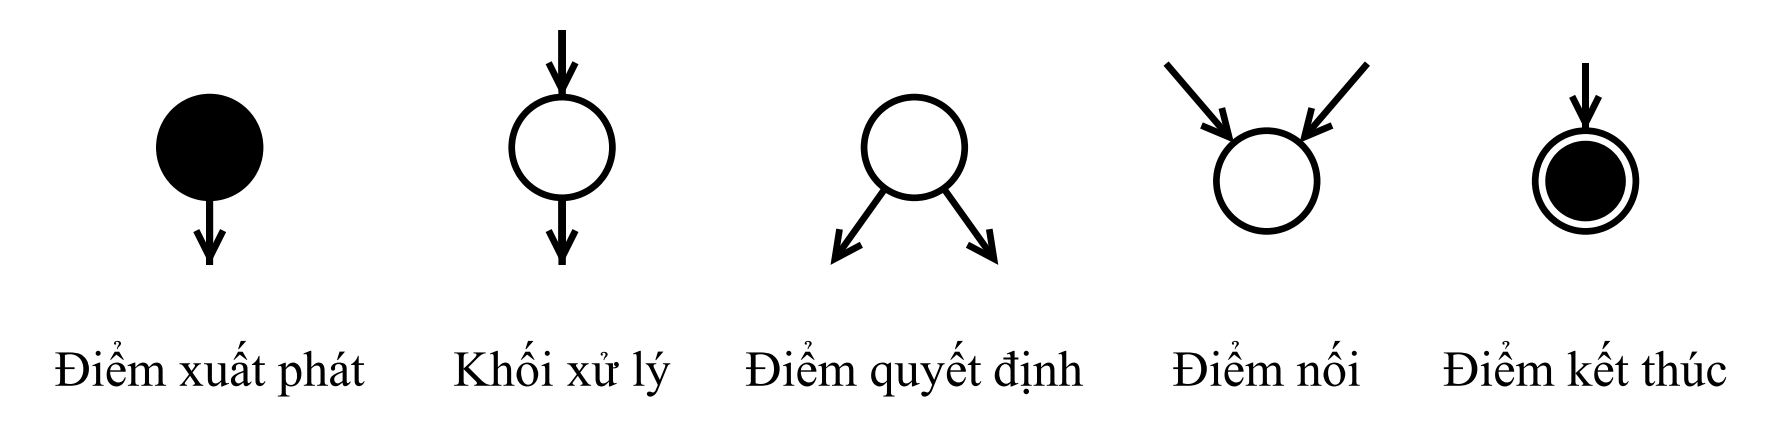
\includegraphics[width=\linewidth]{images/flow-element.png}
	\caption{Các thành phần cơ bản trong đồ thị dòng điều khiển.}
	\label{fig:flow-element}
\end{figure}
\begin{figure}
	\centering
	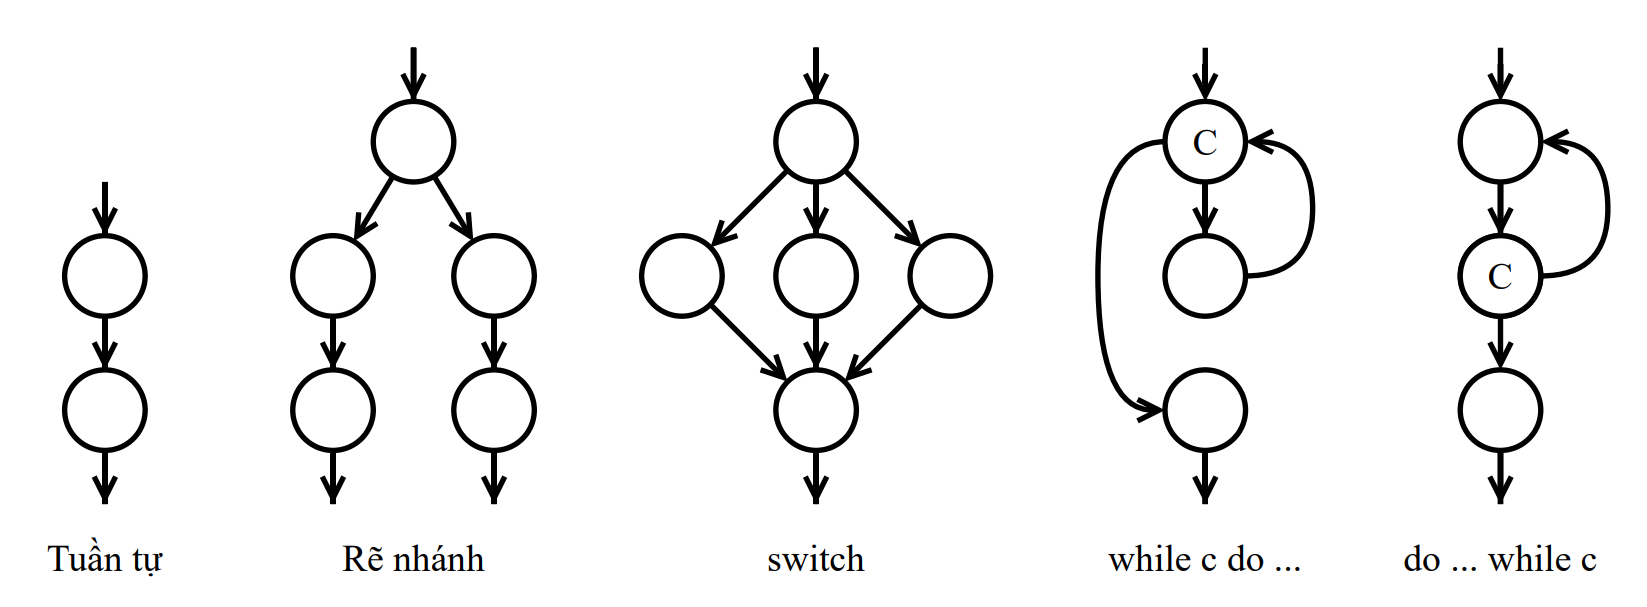
\includegraphics[width=\linewidth]{images/flow-structure.png}
	\caption{Các cấu trúc điều khiển phổ biến trong dồ thị dòng điều khiểnline.}
	\label{fig:flow-structure}
\end{figure}

Đồ thị dòng điều khiển có thể được xây dựng dễ dàng từ AST của mã nguồn. Thông qua việc duyệt tuần tự cấu trúc AST, các đỉnh CFG tương ứng được sinh ra với từng đỉnh biểu thị câu lệnh, điều kiện, vòng lặp, v.v. trên AST.

\section{Đường thi hành}\label{sec:path}
Đường thi hành (Execution Path) là một tập hợp có thứ tự các đỉnh trên CFG thể hiện thứ tự viếng thăm khi thực thi đơn vị kiểm thử tương ứng. Nói cách khác, đường thi hành biểu diễn các câu lệnh được chạy khi thực thi đơn vị kiểm thử với một bộ tham số đầu vào. Định nghĩa chính xác của đường thi hành như sau:

\textbf{Định nghĩa 2.2}\cite{GiaoTrinhKiemThu}: Đường thi hành là một đường đi từ điểm xuất phát đến điểm kết thúc của CFG, được biểu diễn bằng tập hợp các điểm từ $v_1$ đến $v_n$ sao cho cứ hai điểm cạnh nhau thì có cạnh nối theo hướng từ trái qua phải. Nếu cạnh ($v_i$, $v_j$) là nhánh sai thì biểu thức điều kiện tại điểm $v_i$ được viết dưới dạng phủ định $!v_i$.

Đường thi hành có thể chứa rất nhiều câu lệnh và rất nhiều nhánh điều kiện. Điều này dẫn tới việc một đơn vị kiểm thử có thể chứa đường thi hành không khả thi và có thể bùng nổ số lượng đường thi hành. Một đường thi hành không khả thi khi tồn tại những điều kiện không thể thỏa mãn được. Một ví dụ có thể kể đến đó là câu lệnh so sánh \tcode{if(0~==~1)}. Phép so sánh này không bao giờ đúng nên các đỉnh CFG trong nhánh đúng của đỉnh so sánh trên sẽ không thể viếng thăm. Về khả năng bùng nổ số lượng đường thi hành, điều này có thể thấy rõ thông qua các vòng lặp. Các vòng lặp với số lần lặp chưa biết trước có thể tạo ra vô số đường thi hành. Vì vậy việc kiểm thử toàn bộ đường thi hành là một thách thức lớn.

Như vậy, việc sinh dữ liệu kiểm thử cho một đường thi hành tương ứng với quá trình tìm giá trị bộ tham số đầu vào sao cho viếng thăm được toàn bộ đỉnh trên đường thi hành. Trong thực tế, số lượng đường thi hành của một đơn vị kiểm thử có thể rất lớn. Do vậy, việc lựa chọn tập đường thi hành sao cho đạt độ phủ mã nguồn yêu cầu là một thách thức lớn.

\section{Độ phủ mã nguồn} \label{sec:coverage}
Độ phủ mã nguồn là một đơn vị đo số lượng thành phần trong đơn vị kiểm thử được viếng thăm bởi bộ dữ liệu tham số đầu vào. Các thành phần liên quan có thể là câu lệnh, điểm quyết định, điều kiện con, đường thi hành hay là sự kết hợp của chúng \cite{GiaoTrinhKiemThu}. Bộ kiểm thử có độ tin cậy càng cao khi độ phủ đơn vị kiểm thử càng lớn. Ba loại độ phủ mã nguồn được sử dụng phổ biến trong thực tế gồm C1, C2 và C3 \cite{GiaoTrinhKiemThu}. Một số tác giả sử dụng các khái niệm tương ứng gồm Statement, Branch và MCDC (Modified Condition/Decision Coverage). Khóa luận sử dụng khái niệm C1, C2, C3 với định nghĩa như sau:
\begin{itemize}
	\item Độ phủ C1: Được hiểu là độ phủ ở mức câu lệnh, tức mỗi câu lệnh trong đơn vị kiểm thử được thực thi ít nhất một lần sau khi chạy tập ca kiểm thử.
	
	\item Độ phủ C2: Được hiểu là độ phủ ở mức điểm quyết định, tức mỗi điểm quyết định trong CFG của đơn vị kiểm thử đều được thực hiện ít nhất một lần cả nhánh đúng và sai sau khi chạy tập ca kiểm thử.
	
	\item Độ phủ C3: Là độ phủ có điều kiện chặt nhất trong ba loại độ phủ. Điều kiện để đảm bảo độ đo này là các điều kiện con thuộc các điều kiện phức tạp tương ứng với các điểm quyết định trong đồ thị dòng điều khiển của đơn vị cần kiểm thử đều được thực hiện ít nhất một lần cả hai nhánh đúng và sai. Với các phần mềm yêu cầu tính đúng đắn cao, việc sử dụng độ đo C3 để đánh giá mã nguồn là cần thiết.
\end{itemize}

\section{Tập ràng buộc và bộ giải hệ ràng buộc Z3} \label{sec:z3}
Tập ràng buộc là tập các điều kiện mà dữ liệu đầu vào cần thỏa mãn để ca kiểm thử có đường thi hành như mong đợi. Tập ràng buộc được tạo ra bởi tập các điểm quyết định dựa trên kỹ thuật thực thi tượng trưng. Dữ liệu kiểm thử có định hướng cho mỗi đường thi hành được sinh ra bằng cách giải hệ ràng buộc. Trong đó, giải hệ ràng buộc là việc tìm nghiệm cho một tập các ràng buộc được biểu diễn bởi các phép toán điều kiện. Một nghiệm là một tập hợp các giá trị ứng với các biến sao cho tất cả các ràng buộc được thỏa mãn\cite{ref-constraints}. Hiện nay, có nhiều thư viện và công cụ hỗ trợ giải hệ ràng buộc trong đó nổi bật là bộ giải Z3\footnote{https://github.com/Z3Prover/z3}.

Bộ giải Z3 là công cụ được phát triển bởi nhóm Nghiên cứu về Kỹ thuật Phần mềm (RiSE) tại Microsoft Research. Z3 là bộ giải hệ ràng buộc, được xây dựng chủ yếu bằng ngôn ngữ C++. Z3 hỗ trợ giải hệ ràng buộc của các số nguyên, số thực, mảng, hàm tượng trưng, vectơ bit và các biểu thức số học. Công cụ Z3 hỗ trợ định dạng SMT-LIB. Để bộ giải có thể tính toán và giải nghiệm, hệ ràng buộc cần được biểu diễn dưới định dạng SMT-LIB và lưu thành tệp *.smt2. Cấu trúc tệp gồm ba phần chính là phần khai báo, phần định nghĩa các ràng buộc và phần tiện ích. Phần đầu tiên của tệp là phần khai báo, các biến trong hệ ràng buộc được khai báo bằng cú pháp declare-fun <tên biến> () <kiểu dữ liệu>. Tiếp theo, các ràng buộc được thêm bằng cách sử dụng lệnh assert. Phần tiện ích cho phép người dùng sử dụng một số cú pháp có sẵn để thực hiện một số thao tác.

Để giải quyết các đường thi hành chứa các điểm chưa được đi qua của đồ thị dòng điều khiển trong quá trình kiểm thử tượng trưng động, ông Nguyễn Đức Anh và các cộng sự đã đề xuất một phương pháp xử lý. Các đường thi hành trên sẽ được chuyển thành các biểu thức ràng buộc. Sau đó, các biểu thức trên sẽ chuyển thành đầu vào dạng SMT-Lib của bộ giải Z3. Bộ nghiệm đầu ra của Z3 sẽ tương ứng với một đường thi hành trên đồ thị dòng điều khiển. Một tập dữ liệu kiểm thử đạt 100\% độ phủ yêu cầu nếu hệ ràng buộc của các đường thi hành cần thiết cho độ phủ đều giải được.

%\section{Kiểm thử tượng trưng động}

\section{Hàm thiếu định nghĩa} \label{sec:kno-undefine}
\subsection{Tổng quan về hàm thiếu định nghĩa}
Như đã đề cập ở Chương~\ref{chap1}, hàm thiếu định nghĩa là những hàm mà có nguyên mẫu được khai báo, nhưng không có thân hàm (định nghĩa hàm). Để làm rõ hơn khái niệm này, ta cần hiểu thêm về cách khai báo hàm trong ngôn ngữ C/C++. Về cơ bản, một hàm gồm hai phần chính đó là nguyên mẫu hàm và thân hàm. Trong đó, nguyên mẫu hàm thông báo cho trình biên dịch biết tên hàm, kiểu trả về của hàm và danh sách tham số mà hàm nhận. Thân hàm là phần nội dung của hàm nằm trong cặp ngoặc \tcode{\{\}}. Ngôn ngữ C/C++ cung cấp hai cách để người dùng khai báo một hàm (ngoại trừ hàm lambda) gồm khai báo đầy đủ và khai báo tách rời.
\vspace{5mm}
\begin{lstlisting}[language=C++, captionpos=b, caption={Ví dụ về khai báo hàm đầy đủ và khai báo hàm tách rời.}, label={cod:kno-undef}]
// Full function declaration
int foo(int a, int b) {
	return a + b;
}
// Function prototype + Function defintion 
int bar(int a, int b);
int echo(double);
int main() { bar(1,2); }

int bar(int a, int b) {
	return a - b;	
}
\end{lstlisting}

Đoạn mã \ref{cod:kno-undef} minh họa ví dụ về khai báo đầy đủ và khai báo tách rời. Dòng 1-3 thể hiện khai báo tách rời của hàm \tcode{foo} với nguyên mẫu hàm và thân hàm đều nằm trong cùng một câu lệnh khai báo. Dòng 6 thể hiện khai báo nguyên mẫu hàm của hàm \tcode{bar} và cho biết hàm này trả về giá trị kiểu \tcode{int} và nhận hai tham số đầu vào kiểu \tcode{int}. Dòng 7 cũng thể hiện nguyên mẫu hàm \tcode{echo}. Dòng 11-13 thể hiện khai báo định nghĩa hàm (thân hàm) của hàm \tcode{bar}.

Nguyên mẫu hàm là một trong những tính năng quan trọng của ngôn ngữ C/C++. Nguyên mẫu hàm cung cấp cho trình biên dịch biết những thông tin cơ bản của hàm và trình biên dịch ngầm hiểu rằng định nghĩa của hàm này có tồn tại. Cơ chế này giúp tăng tính tái sử dụng mã nguồn trong ngôn ngữ C/C++. Thông qua việc khai báo nguyên mẫu hàm trong các tệp header, người dùng có thể tái sử dụng các hàm mà không cần biết chi tiết nội dung bên trong hàm đó.

Nguyên mẫu hàm là một tính năng hữu ích song nó cũng có nhược điểm. Nhược điểm của tính năng này đó là sự phụ thuộc vào người dùng. Một nguyên mẫu hàm không cần thiết phải có định nghĩa hàm bởi có thể nó không được sử dụng trong mã nguồn. Với ví dụ trong Đoạn mã~\ref{cod:kno-undef}, nguyên mẫu hàm \tcode{echo} không cần có định nghĩa bởi nó không được sử dụng trong bất kì thành phần nào khác. Trình biên dịch có khả năng tự xác định các nguyên mẫu hàm được sử dụng khi phân tích cú pháp mã nguồn ở bước biên dịch. Quá trình liên kết các tệp đối tượng có mục đích xác định định nghĩa hàm tương ứng với từng nguyên mẫu hàm. Ở bước này, nếu trình biên dịch không thể tìm thấy định nghĩa hàm tương ứng, nguyên mẫu hàm được coi là hàm thiếu định nghĩa.
\subsection{Nguyên mẫu hàm ảo và lỗi thiếu bảng ký hiệu ảo}
Hàm ảo là một cơ chế mới được giới thiệu trong ngôn ngữ C++ nhằm thể hiện các đặc trưng hướng đối tượng so với ngôn ngữ C. Hàm ảo là một hàm đặc biệt, chỉ có thể khai báo trong lớp và có khả năng ghi đè bởi hàm ở lớp dẫn xuất. Khi hàm ảo ở lớp cơ sở được gọi, chương trình sẽ tự động hiểu và chọn đúng đối tượng ở lớp dẫn xuất để gọi đúng hàm ghi đè. Khả năng trên được gọi là đa hình. Nguyên mẫu hàm ảo cũng có các đặc điểm tương tự như nguyên mẫu hàm bình thường.

Để có được khả năng đa hình, ngôn ngữ C++ giới thiệu một khái niệm mới có tên là bảng ký hiệu ảo (Vtable). Vtable là bảng lưu trữ các khai báo biến, hàm có trong một kiểu dữ liệu tự định nghĩa do trình biên dịch tạo ra khi biên dịch một tệp mã nguồn. Vtable là công cụ giúp trình biên dịch biết một biến đã được định nghĩa hay chưa, biến đó thuộc kiểu gì, từ đó thông báo đến người dùng nếu có lỗi ngữ pháp. Vtable còn là công cụ giúp chương trình xác định được hàm nào sẽ được thực thi bằng cách sử dụng cơ chế liên kết động. Nếu hàm ảo, thuần ảo thiếu định nghĩa hàm thì khi liên kết, trình biên dịch sẽ báo lỗi do không biết chương trình sẽ cần hàm nào để chạy. Khác với các nguyên mẫu hàm bình thường, trình biên dịch không hiển thị lỗi hàm thiếu định nghĩa nếu không tìm thấy định nghĩa của hàm ảo mà sẽ hiển thị lỗi thiếu bảng ký hiệu ảo. Nguyên nhân gây ra lỗi này là bởi trình biên dịch không cho phép gọi hàm ảo nếu nó không có ít nhất một hàm ghi đè.

Để làm rõ hơn ví dụ về lỗi thiếu bảng ký hiệu ảo, ta xét ví dụ trong Đoạn mã~\ref{cod:kno-vtable}. Đoạn mã này chứa hai lớp \tcode{A} và \tcode{B} trong đó \tcode{B} là lớp dẫn xuất của \tcode{A}. Lớp \tcode{A} có chứa ba nguyên mẫu hàm ảo, trong đó hàm~\tcode{bar} được ghi đè ở lớp dẫn xuât và hàm~\tcode{echo} là khai báo hàm ảo đầy đủ. Trong quá trình liên kết để tạo thành tệp thực thi, trình biên dịch báo lỗi thiếu Vtable cho kiểu \tcode{A} bởi trình biên dịch không thể tìm thấy hàm ghi đè nguyên mẫu hàm ảo \tcode{foo} ở lớp dẫn xuất.

\vspace{5mm}
\begin{lstlisting}[language=C++, captionpos=b, caption={Ví dụ về lỗi thiếu bảng ký hiệu ảo.}, label={cod:kno-vtable}]
class A {
	virtual int echo() {}
	virtual int foo();
	virtual int bar();
};
class B : public A {
	int bar() {}
}
\end{lstlisting}
\subsection{Vai trò trong các dự án C/C++}
Nguyên mẫu hàm đóng vai trò quan trọng trong các dự án C/C++ khi nó cho phép người dùng tái sử dụng mã nguồn. Trong quá trình phát triển phần mềm, nguyên mẫu hàm cho phép các thành viên trong nhóm phát triển đặt ra những lớp giao diện, các hành vi sẽ được cung cấp bởi mô-đun họ phụ trách. Điều này thúc đẩy quá trình phát triển phần mềm nhanh hơn bởi các thành viên không cần phải đợi sự hoàn thiện từ các thành phần phụ thuộc. Do quá trình kiểm thử đơn vị diễn ra song song với quá trình phát triển nên ta không thể tránh khỏi tình trạng mã nguồn tồn tại một số nguyên mẫu hàm thiếu định nghĩa. Vì vậy, nhu cầu phát triển một giải pháp kiểm thử tự động đặc biệt cho mã nguồn C/C++ chứa hàm thiếu định nghĩa là vô cùng thiết yếu. Theo khảo sát của khóa luận về phương pháp xử lý hàm thiếu định nghĩa, hiện chưa có phương pháp nào được đề xuất vậy nên khóa luận sẽ thảo luận chi tiết về phương pháp giải quyết ở Chương~\ref{chap3}.

\section{Sinh giả lập mã nguồn tự động} \label{sec:autostub-Lam}
Việc sinh giả lập mã nguồn tự động trở thành một bài toán quan trọng khi các đơn vị kiểm thử có chứa các lời gọi hàm đến các chức năng khác trong mã nguồn chưa hoàn thành vì các giai đoạn kiểm thử và phát triển thường được thực hiện song song. Một số phương pháp sinh stub tự động đã được đề xuất để giải quyết bài toán trên. Trong đó, phương pháp AS4UT~\cite{TUNG2022106821} năm 2022 được đề xuất để sinh stub được sử dụng trong kiểm thử đơn vị các dự án C/C++. Ý tưởng chính của AS4UT là coi mỗi lời gọi hàm là một biến giả. Ý tưởng được thực hiện bằng cách thêm giai đoạn tiền xử lý đồ thị dòng điều khiển CFG vào hướng tiếp cận kiểm thử tượng trưng động. Trong giai đoạn tiền xử lý, tất cả các lời gọi hàm trong CFG của đơn vị được kiểm thử được thay thế bằng các biến giả tương ứng. Sau đó, CFG đã biến đổi được sử dụng làm đầu vào để tạo tập dữ liệu kiểm thử. Tuy nhiên, phương pháp AS4UT hiện tại chỉ chú trọng vào kết quả trả về của lời gọi hàm mà chưa quan tâm tới sự thay đổi nếu đó là lời gọi phương thức. Điều này có thể gây khó khăn khi kiểm thử các đơn vị có nhiều sự tương tác của các đội tượng bởi lời gọi phương thức có thể thay đổi gía trị thuộc tính của đối tượng.